\documentclass{article}
\usepackage[utf8]{inputenc}
\usepackage{graphicx}
\usepackage{hyperref}
\usepackage{float}
\usepackage{csvsimple}

\begin{filecontents*}{scientists.csv}
Lambda(nm),Couleur œil nu,Couleur Iphone
390,Invisible,Bleu foncé assez faible
400,Violet foncé faible intensité,Violet faible
410,Violet foncé,Violet foncé
420,Violet foncé,Violet foncé
430,Violet foncé,Violet foncé
440,Bleu Foncé,Violet pale
450,Bleu Foncé,bleu foncé
460,bleu foncé,bleu foncé
470,bleu un peu moins foncé,bleu un peu moins foncé
500,Vert bleuté,Vert bleuté
520,Vert pomme,Vert pomme
540,Vert clair,Vert clair
560,Vert morve,Vert morve
580,Orange soleil ,Orange soleil
600,Orange crépuscule,Orange crépuscule
620,Rouge,Rouge
640,Rouge,rouge rosé
660,Rouge moins lumineux,Rose rouge
680,Rouge peu lumineux,Rosé
700,Bordeaux,Rouge foncé
720,Rouge peu visible,Faible bordeaux
740,Bordeaux très peu visible,Très faible bordeaux
760,Rouge presque invisible,Très faible bordeaux
780,Invisible,Invisible
800,Violet,Violet
850,Bleu foncé faible,Bleu foncé faible
900,Bleu foncé,Bleu foncé
950,turquoise faible,turquoise faible
1000,Vert turquoise,Vert turquoise
1050,Vert faible,Vert faible
1100,Vert jaune,Vert jaune
\end{filecontents*}

\title{TP sur les capteurs optiques}
\author{Hocine ABDELHAMID : 21100727}
\date{November 2022}

\begin{document}

\maketitle

\section{Introduction}
Le but du TP est d'étudier la réponse spectral d'un capteur monochrome CCD et d'un capteur monochrome CMOS dans un premier temps, puis d'étudier le bruit temporel et le bruit spatial fixe du capteur dans un second temps. Pour ce faire nous allons utiliser un système composé d'une lampe halogène, un monochromateur, une sphère intégratrice, un capteur calibré et le capteur sous test. Nous allons dans un premier temps présenter ce matériel puis vous présenter nos résultats.

\section{Présentation du matériel}

\begin{figure}[H]
\centering
\includegraphics[scale=0.5]{schéma_dispo.png}
\label{fig:4}
\caption{Schéma du dispositif}
\end{figure}

\subsection{Le monochromateur}
Le monochromateur (voir figure \ref{fig:1}) est un dispositif optique qui sépare la lumière polychromatique. Un jeu de miroir couplé à un réseau de diffraction permet de séparer les différentes longueur d'ondes de la lumière émise par la lampe halogène. Au final, une fente laisse passer seulement la longueur d'onde sélectionnée (grâce a un logiciel) dans la sphère intégratrice \ref{fig:2}.



\subsection{Source de lumière}
La lumière est émise par une lampe halogène. Elle est émise de sorte que les rayons arrivent a peu près parallèle avant d'être traité par le monochromateur

\begin{figure}[H]
\centering
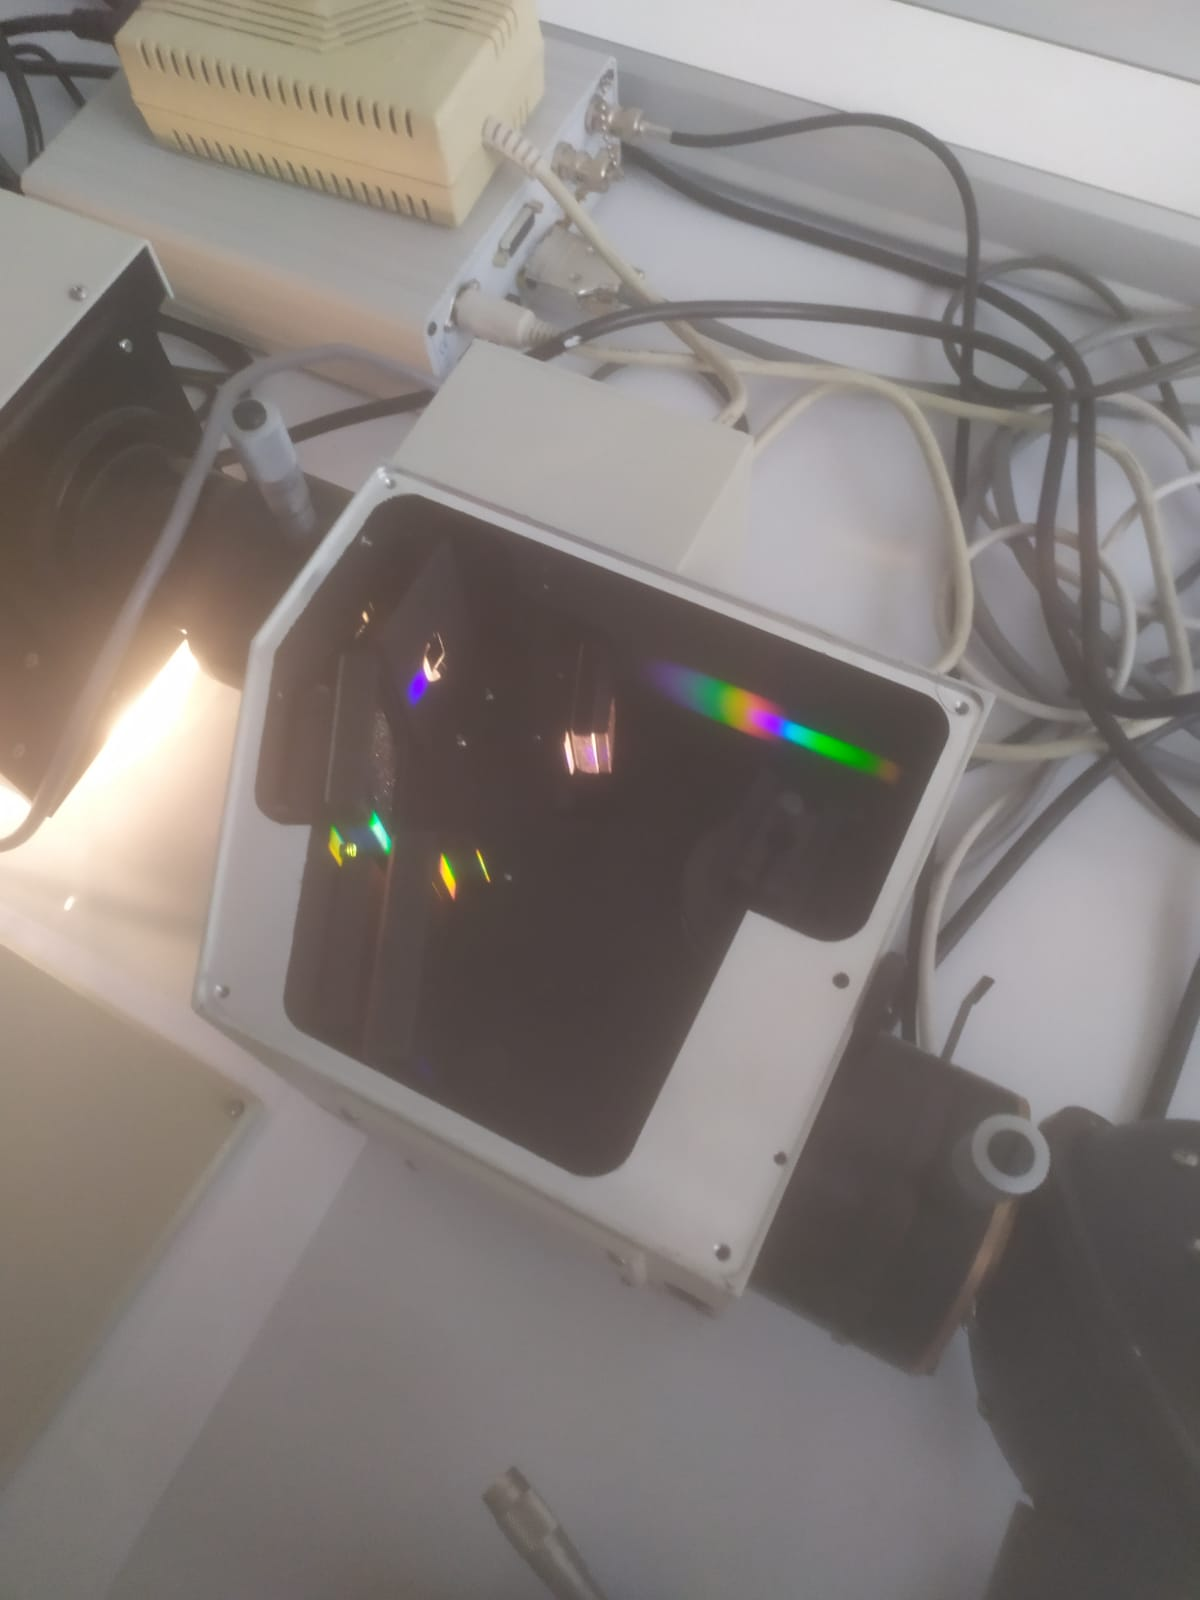
\includegraphics[scale=0.2]{monochromateur.jpg}
\label{fig:1}
\caption{monochromateur}
\end{figure}

\begin{figure}[H]
\centering
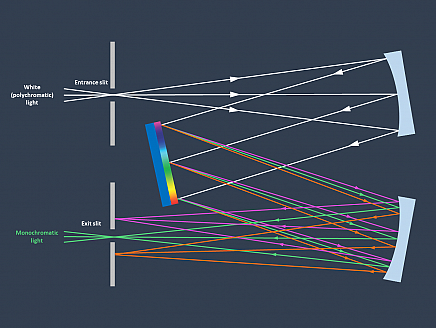
\includegraphics[scale=0.7]{monochromateur_principe.png}
\label{fig:2}
\caption{principe du monochromateur}
\end{figure}

\begin{figure}[H]
\centering
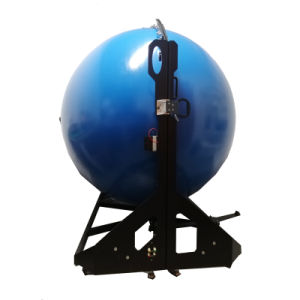
\includegraphics[scale=0.7]{sphere_integrante.jpg}
\label{fig:3}
\caption{sphère intégratrice}
\end{figure}

\subsection{Sphère intégratrice}
La sphère intégratrice \ref{fig:3} a pour fonction de diffuser la lumière équitablement dans toutes les direction. On dit que c'est un diffuseur parfait. Elle diffuse la lumière de sorte que l'intensité lumineuse soit la même pour le détecteur calibré et pour le capteur sous test.


\section{Les capteurs}
\subsection{Capteurs CCD vs capteurs CMOS}
Dans un premier temps, il fallait déterminer quels sont les capteurs CCD et les capteurs CMOS.
une différence notable entre ces deux capteurs est que le CMOS intègre pour chaque pixel une photo-diode (qui sert a la conversion photon-charge et au stockage des charges) ainsi qu'un amplificateur qui permet la conversion des charges en tension. Autrement dit le capteur CMOS fais l'acquisition de la lumière et la conversion en tension au sein même de la puce, ce qui rend, par rapport au CCD, un circuit plus compacte et par extension, moins lourd.
Une autre différence est le fait que les photo-diodes du capteur CMOS peuvent être constituée d'un autre matériaux que le silicium. Et cela permet par exemple d'utiliser le capteur CMOS sur une grande étendue de longueur d'ondes. 

\subsection{Capteur noir et blanc capteurs couleurs}
Il existe plusieurs techniques pour pouvoir retranscrire les couleurs. On va développer ici le filtre de Bayer.
Dans le filtre de bayer, on ajoute sur chaque photo-site un filtres rouge, vert ou bleu. on obtient une mosaïque de 4 filtres : 2 vert, 1 rouge, 1 bleu.

\begin{figure}[H]
\centering
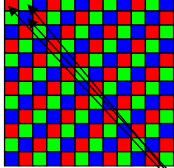
\includegraphics[scale=0.7]{mosaique_filtre.png}
\label{fig:mosaique}
\caption{Mosaïque de filtre, 2 vert, 1 rouge, 1 bleu}
\end{figure}

La raison pour laquelle on utilise plus de filtre vert que de filtre bleu et rouge est que l'oeil humain possède plus de cône vert que de cône rouge et bleu. Il capte par conséquent mieux la lumière verte.

\section{Utilisation du monochromateur}
On teste le monochromatueur sur différente longueur d'onde dans le domaine du visible.
on a fait un tableau présentant la couleur observée dans la sphère en fonction de la longueur d'onde à l'oeil nu, et avec notre téléphone.
\begin{table}[H]
\csvautotabular{scientists.csv}
\caption{Couler en fonction de lmabda}
\label{tab:lambda}
\end{table}

On voit par moment, principalement dans l'ultraviolet, que l'iphone capte une couleur légèrement différente qua' l'oeil nu. En effet l'iphone embarque un capteur CMOS avec un post traitement qui créer ces différences.
On voit également que dans l'infrarouge, on peut observer a l'oeil nu, une couuleur dans la sphère. 
Cela corresepond a la deuxieme frange d'interference du au réseau de diffraction. Une solution pour éviter cela est d'utiliser un filtre passe haut afin de couper les longueur d'ondes indésirables.

\section{Mesure de la réponse spectral}
Après avoir calibré les paramètres images de la caméra de sorte a ce qu'elle ne sature pas (choix d'un temps d'exposition de 200ms pour environ 4fps), on a enregistré pour chaque longueur d'ondes une trentaine d'image pendant que le détecteur calibré effectuait les mesures de la tension.
On a ensuite écrit un programme afin de calculer la valeur moyenne des mesures a chauqe longueur d'ondes du deteceur calibré, ainsi que l'image moyenne des 30 images. (le code est disponible sur le lien suivant : \url{https://github.com/Huss94/capteurs-optiques})

\subsection{Calcul de la puissance lumineuse moyenne}
Dans un premier temps on calcule la moyenne a chaque longueur d'onde de la valeur numérique donnée par le detecteur calibré. On obtient un tableau contenant pour chaque longueur d'onde, une valeur moyenne.
On divise ensuite ces valeurs par la réponse spectral du détecteur calibré.
\begin{figure}[H]
\centering
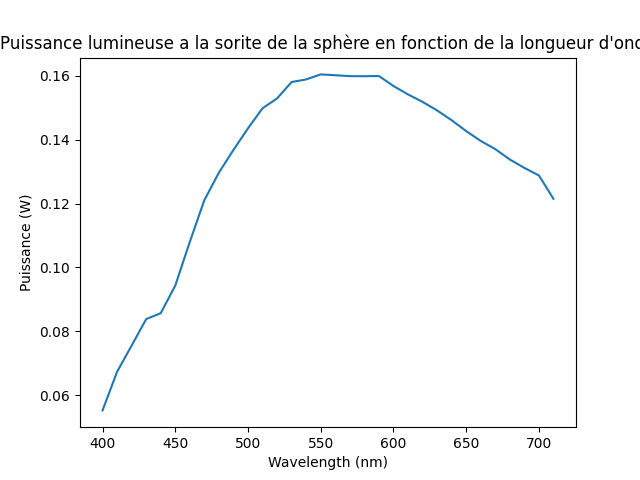
\includegraphics[scale=0.7]{puissacnes.png}
\label{fig:mosaique}
\caption{Puissances moyennes en fonction de la longueur d'onde}
\end{figure}

On remarque que la puissance est la plus élevé en 550nm ce qui est caractéristique du silicium.

Il faut maintenant calculer la réponse spectral du CCD. On va utiliser pour cela les images moyennes calculé précédemment qui représentent la valeur numérique moyenne
La réponse spectral a une longueur d'onde donnée est alors  $$Rs = \frac{Vn}{P}$$
où Vn est la valeur numérique te P la puissance lumineuse. \\
Nous avons des images moyennes on va alors calculer la réponse spectrale de 3 manière différentes : \\
    - Sur un seul pixel \ref{fig:pixel} \\
    - Sur une petite fenetre de l'image \ref{fig:fenetre} \\
    - Sur toute l'image \ref{fig:full_img} \\
  
\begin{figure}[H]
\centering
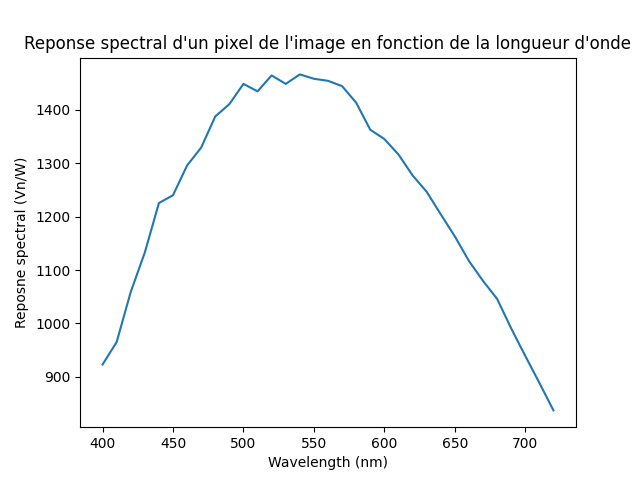
\includegraphics[scale=0.7]{pixel.png}
\label{fig:pixel}
\caption{Reponse spectral d'un seul pixel de l'image en fonction de la longueur d'onde}
\end{figure}

\begin{figure}[H]
\centering
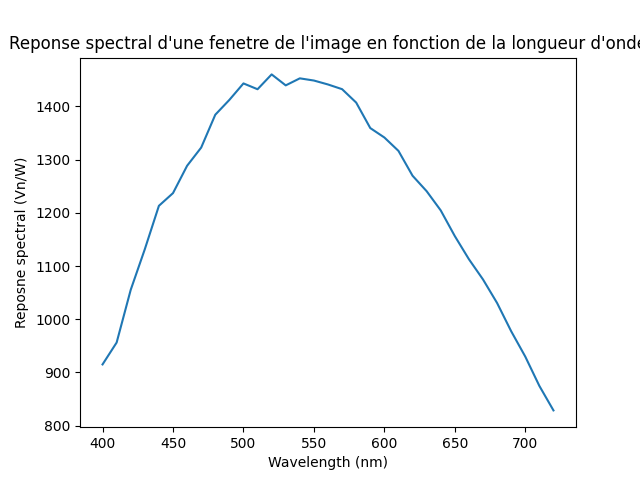
\includegraphics[scale=0.7]{fenetre.png}
\label{fig:fenetre}
\caption{Reponse spectral d'une fenetre de l'image en fonction de la longueur d'onde}
\end{figure}

\begin{figure}[H]
\centering
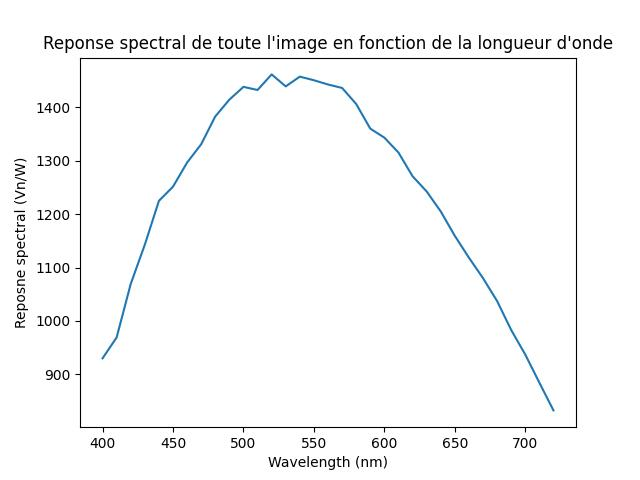
\includegraphics[scale=0.7]{full_img.jpg}
\label{fig:full_img}
\caption{Reponse spectral de toute l'image en fonction de la longueur d'onde}
\end{figure}

\section{Bruit temporel et bruit spatial}

Nous n'avons pas eu le temps en TP de prendre les 100 images nécessessaire à cette partie, on va cependant utiliser les 30 images prises pour la partie précédente.

On trace la valeur d'un pixel en fonction du temps afin de visualiser le bruit temporel. \ref{fig:bruit_temporel}


\begin{figure}[H]
\centering
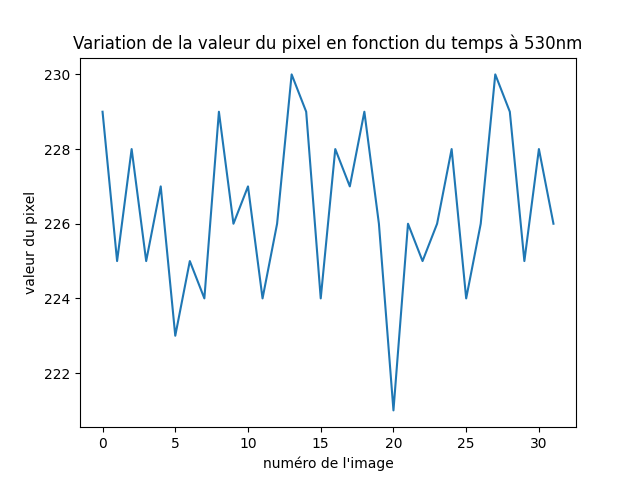
\includegraphics[scale=0.7]{bruit_temporel.png}
\label{fig:bruit_temporel}
\caption{Bruit temporel pour les images prisent à $\lambda$ = 530nm}
\end{figure}


Pour le bruit spatial fixe, on calcul la moyenne des images à 530nm et on trace chaque pixel de l'image  \ref{fig:BSF}


\begin{figure}[H]
\centering
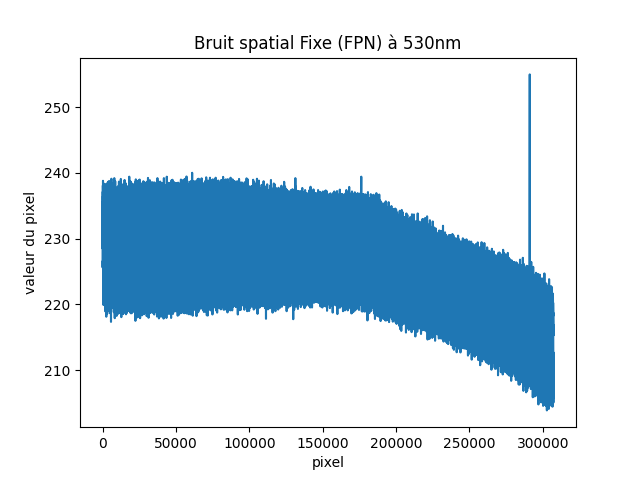
\includegraphics[scale=0.7]{bruit_spatial_fixe.png}
\label{fig:BSF}
\caption{Bruit spatial fixe pour l'image moyenne à $\lambda$ = 530nm}
\end{figure}

ces bruits peuvent être dû aux interférences électromagnétiques, aux bruit thermique (courant noir) et plusieurs autres facteurs.


\end{document}





